\chapter{Application and Results}
\label{chap:app}

To verify the proposed Qualitative Control Theory, we test our method for motion synthesis.

At current, the objective is not generating a fully detailed character animation, but to develop practical routines and tools for full body animation.

Within QCF framework, this test includes three steps:
\begin{enumerate}
\item identify the topological structure of the motion
\item test the structure stability.
\item change the controller parameters, build a repertoire of parameters
\end{enumerate}

In the following sections, three examples are shown. 
The first two are one degree systems, the mass spring system and bouncing ball system. 
One degree system is the building block for complex systems. 
The two examples are the simplest continuous system and discontinue system. 
We show that after coupling with the neural oscillator, 
we change the original system into structural stable autonomous system.

The third example is more complex and meaningful. 
It is a 2D biped walking example.
The coupling of neural oscillator turned the original passive walking into a more stable autonomous system.
Natural looking gaits with adaptation are generated by this method.

\section{One Degree Of Freedom Systems}
The first system is the mass-spring-damping system controlled by a nonlinear oscillator. 
For CMS, this example captures the essence of interaction between bones, muscles and neural systems. 
In this system, bones are simplified as mass; muscles are modelled as springs with damping effects. 
Neural oscillator simulates the effects of neural system. This idea can be extended to deal with more complex situations.
Mass spring system can be used to model system with continuous dynamic properties. 
Typical example includes arm swing and posture control.

%the coupled mass-spring and neural oscillator system.
%following is a figure of mass-spring damping system
%\begin{figure}
%\end{figure}
\subsection{Simulation Method of Mass Spring System}
Mathematically, Forced mass spring system is formulated as equation \eqref{equ:mass-spring-damping}
\begin{equation}
\ddot{x}+K(x-x_{os})+D\dot{x}=0
\label{equ:mass-spring-damping}
\end{equation}

It is a forced spring damping system. 
The driven force $x_{os}$ is determined by the neural oscillator.
\begin{equation}
x_{os}=H_{out}*y_{out}
\end{equation}
where $H_{out}$ is the couple coefficient  between neural oscillator output and the mass-spring input. 
The neural oscillator is defined by equation \eqref{eq:matsuta}.


The state values of spring damping system will be sent back to the neural oscillator as described in the following equation.
\begin{eqnarray}
g_{1}=h_{i1}*x\\
g_{2}=h_{i2}*\dot{x}
\end{eqnarray} 
where $h_{i1}$ and $h_{i2}$ determines the coupling between mechanical system and controller, $g_{1} , g_{2}$ are feed to the neural oscillator.

The uncoupled spring damping system shows nearly periodic behaviour. 
Its trajectories terminate at the position $(0,0)$ as showed in Figure ~\ref{fig:spring-damping oscilaor}.
\begin{figure}
\begin{center}
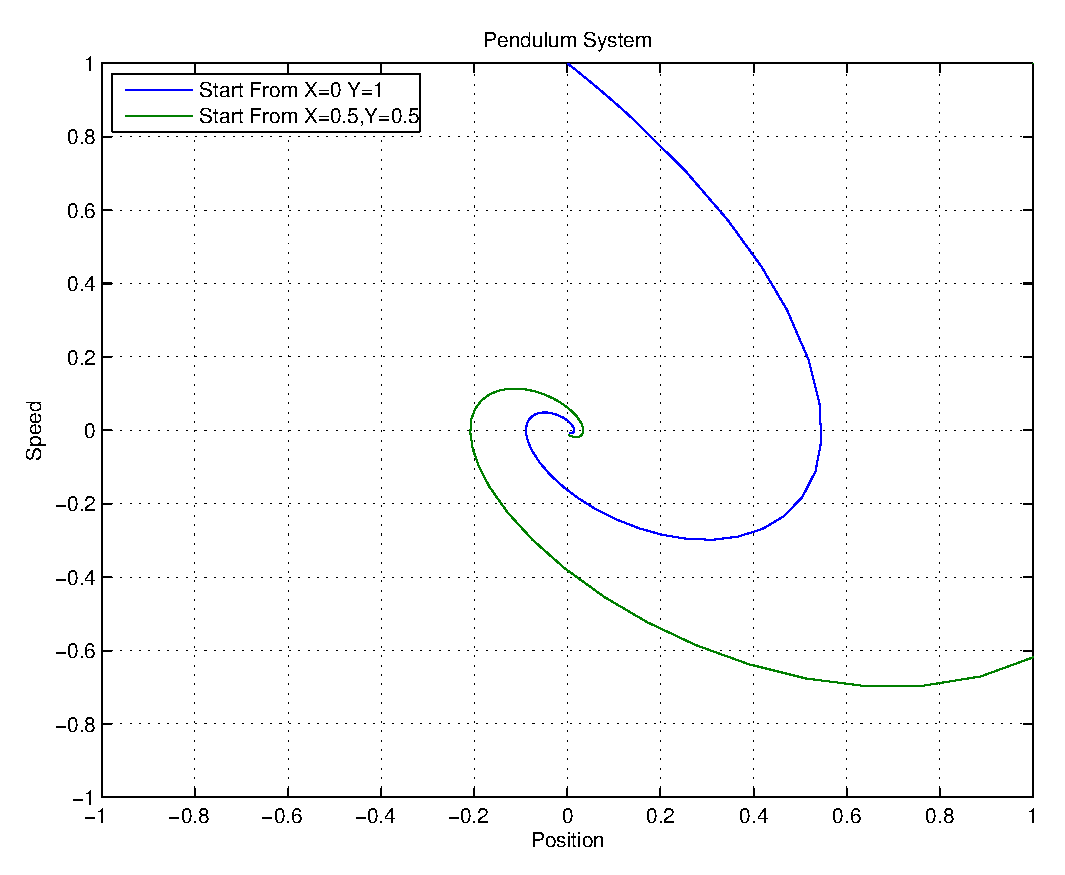
\includegraphics[width=0.6\textwidth]{\figurepath/spring_damping.eps}
\end{center}
\caption{the trajectory of the damping system}
\label{fig:spring-damping oscilaor}
\end{figure}

In our simulation, the motion equation above will be discretized and integrated with runge-kutta method\citep{Press1992}.
\subsection{Simulation Result}
After being coupled with the neural oscillator, this mass spring system shows a different topology structure. 
This gives the system stability and adaptive power.
Motion trajectories with different initial condition converged to the same limited circle. 
The trajectory of the limited circle resembles to that of the original motion. 
Figure ~\ref{fig:spring-damping entraint oscilaor} shows the states of the system overtime, and Figure ~\ref{fig:spring-damping entraint oscilaor phase} shows the phase plot.

\begin{figure}
\begin{center}
	\subfigure[state plot]
	{
	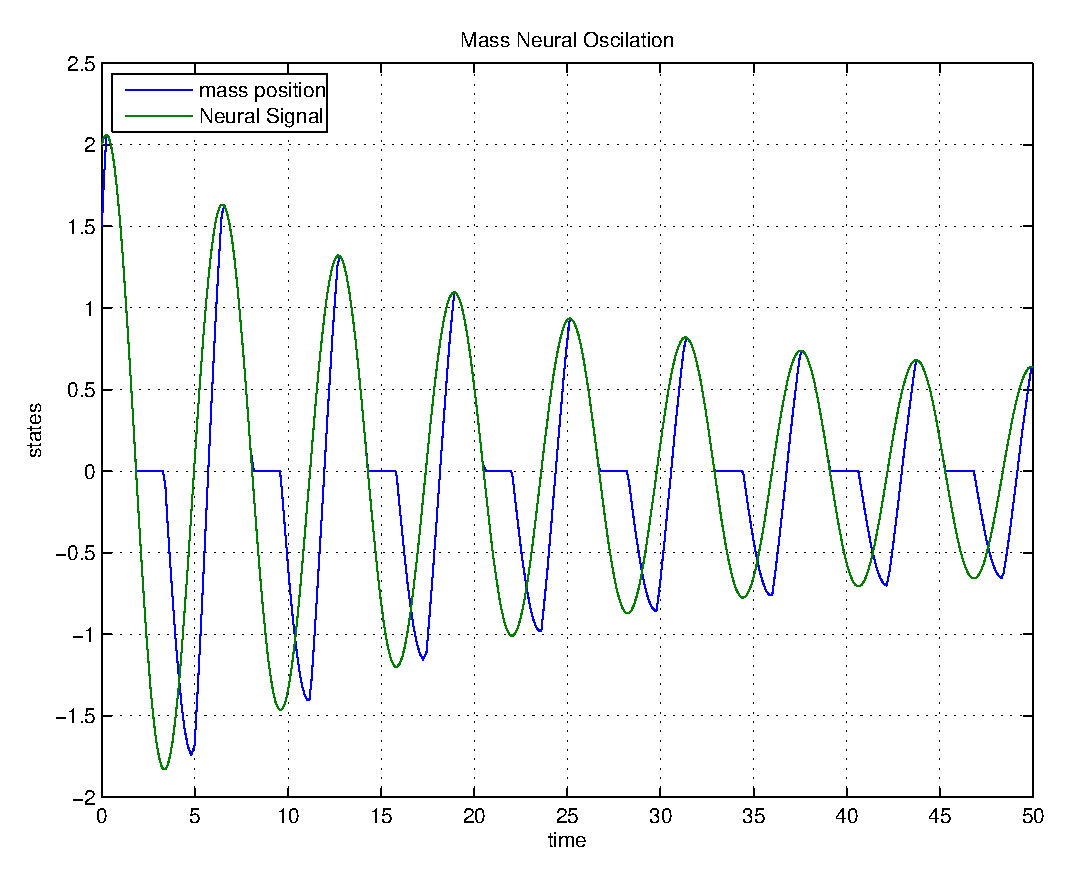
\includegraphics[width=0.45\textwidth]{\figurepath/mass_neural_entraint.eps}
	\label{fig:spring-damping entraint oscilaor}
	}
	\subfigure[Phase Plane]
	{
	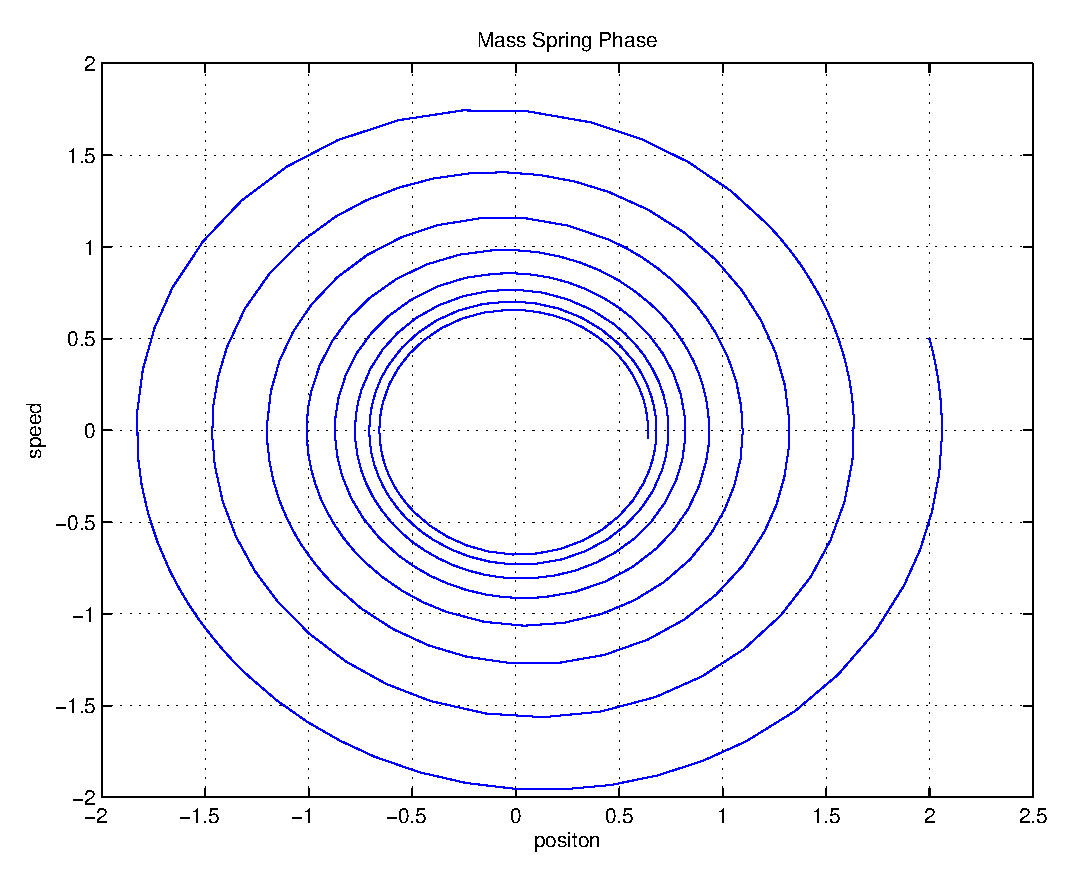
\includegraphics[width=0.45\textwidth]{\figurepath/mass_neural_mass_phase.eps}
	\label{fig:spring-damping entraint oscilaor phase}
	}
	\caption{Mass spring system coupled with a neural oscillator}
\end{center}
\end{figure}

From Figure ~\ref{fig:attractive circle}, we found that the limit circle is attractive and basin of attraction of this system covers a large area.

\begin{figure}
\begin{center}
	\subfigure[state plot]
	{
	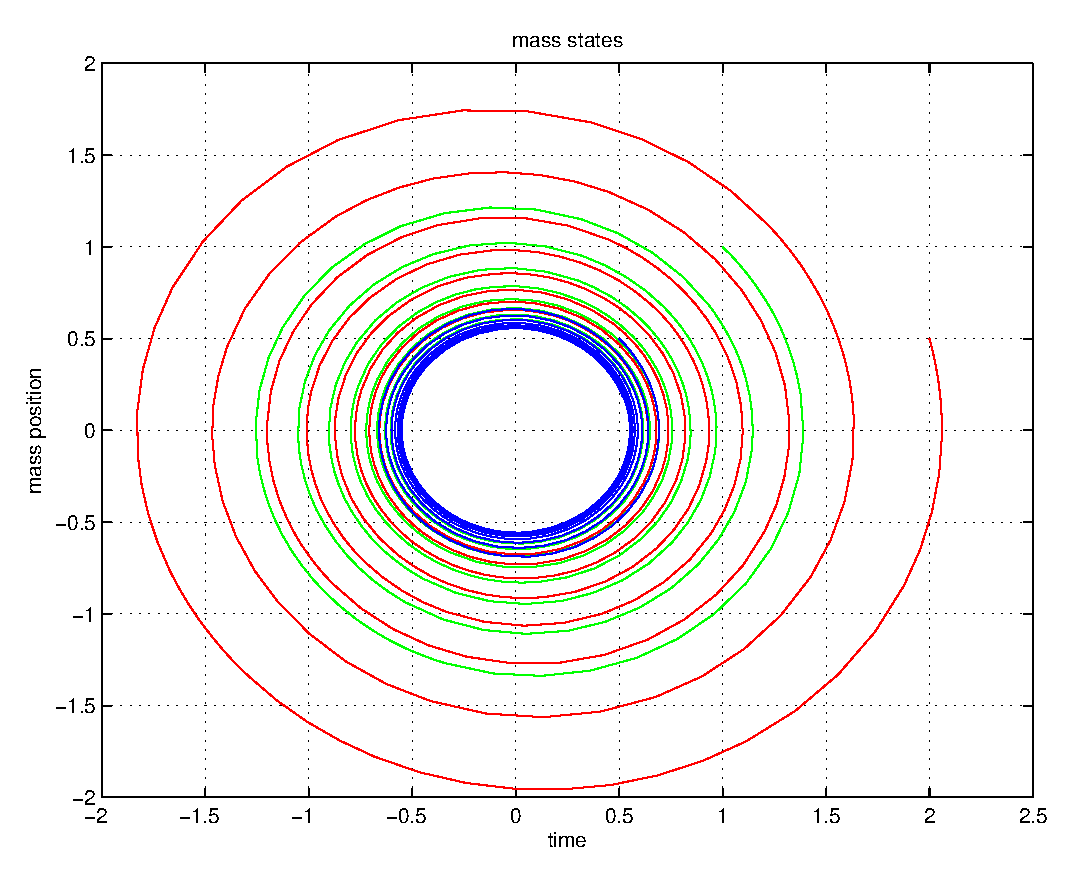
\includegraphics[width=0.45\textwidth]{\figurepath/mass_state_attraction_phase.eps}
	\label{fig:attractive-spring-damping entraint oscilaor}
	}
	\subfigure[Phase Plane]
	{
	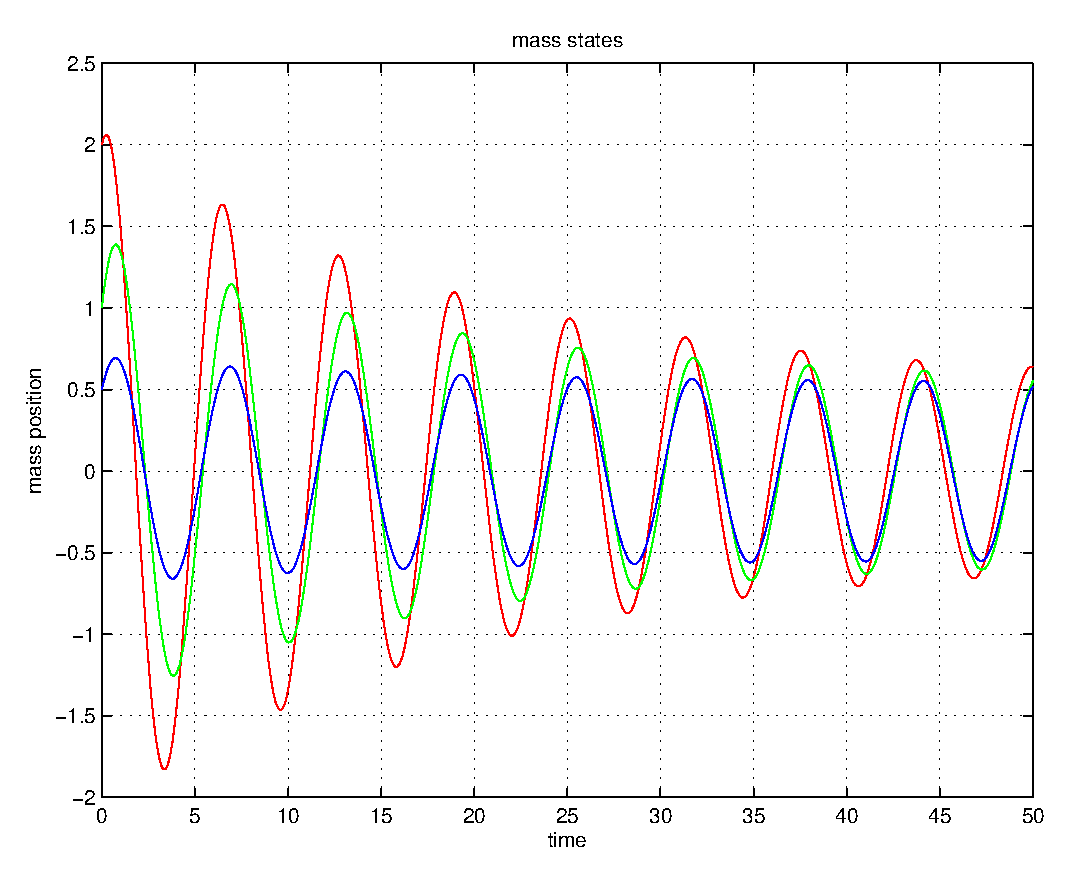
\includegraphics[width=0.45\textwidth]{\figurepath/mass_state_attraction.eps}
	\label{fig:attractive-spring-damping entraint oscilaor phase}	
	}
	\caption{Attractive Limited Circle}
	\label{fig:attractive circle}
\end{center}
\end{figure}

\subsection{Effects of Parameter Turning}
\begin{description}
\item[Increasing sensing coefficient $H$], the final oscillation will be close to mechanical oscillation.
\item[Increasing $H_{out}$], the final oscillation frequency will turn close to neural oscillation.
\item[Increasing $c$ of the neural oscillator], this will increase oscillation amplitude. It will not affect the frequency.
\item [Increasing $\tau_{1}$], the frequency of oscillation will be changed. And there exists an optimal frequency$\tau _{max}$. No matter the frequency becomes larger or smaller than that optimal value, the oscillation magnitude will be lower.
\end{description}

\subsection{Bouncing Ball System Simulation}

The second example is a bouncing ball driven by a neural oscillator. 
This example captures the essence of complex interaction between body and environment. 
In CMS, the idea can be extended for simulating throw and catch, jumping, running, jiggling and walking. 
In our research, we found out that the neural oscillator is a very simple but robust way to control motion.

When the ball is flying in the air, the motion of the ball can be easily described with 
\[
\ddot{x}=g ,x>x_{ground}
\]
When ball hit a moving object, we assume that collision happens in short time. We apply an impulse to the ball.
\[
\dot{x}_{+}=-e(\dot{x}-\dot{x}_{ground})+\dot{x}_{ground}
\]

Because the ground is fixed, the natural topological structure shows nearly periodic behaviour showed in Figure ~\ref{fig:bounce-ball}

\subsection{Adaptive Motion for Bouncing Ball System}
Although these bouncing ball system and mass spring system are very different, bouncing ball system has the same topological structure with the damping spring mass system. 
Thus the bouncing ball system can be seen as a nonlinear mass spring.

When it is coupled with a neural oscillator, the ground position $x_{ground}$ is driven by the neural oscillator, and the speed $\dot{x}$ will be feedback to the neural oscillator as input signal. 
Similar to the mass spring system, the bouncing ball system converge to an attractive limit circle. 
The entrainment behaviour is plotted in Figure ~\ref{fig:fig_bb_entraint}.

\begin{figure}[h]
\begin{center}
	\subfigure[state plot]
	{
	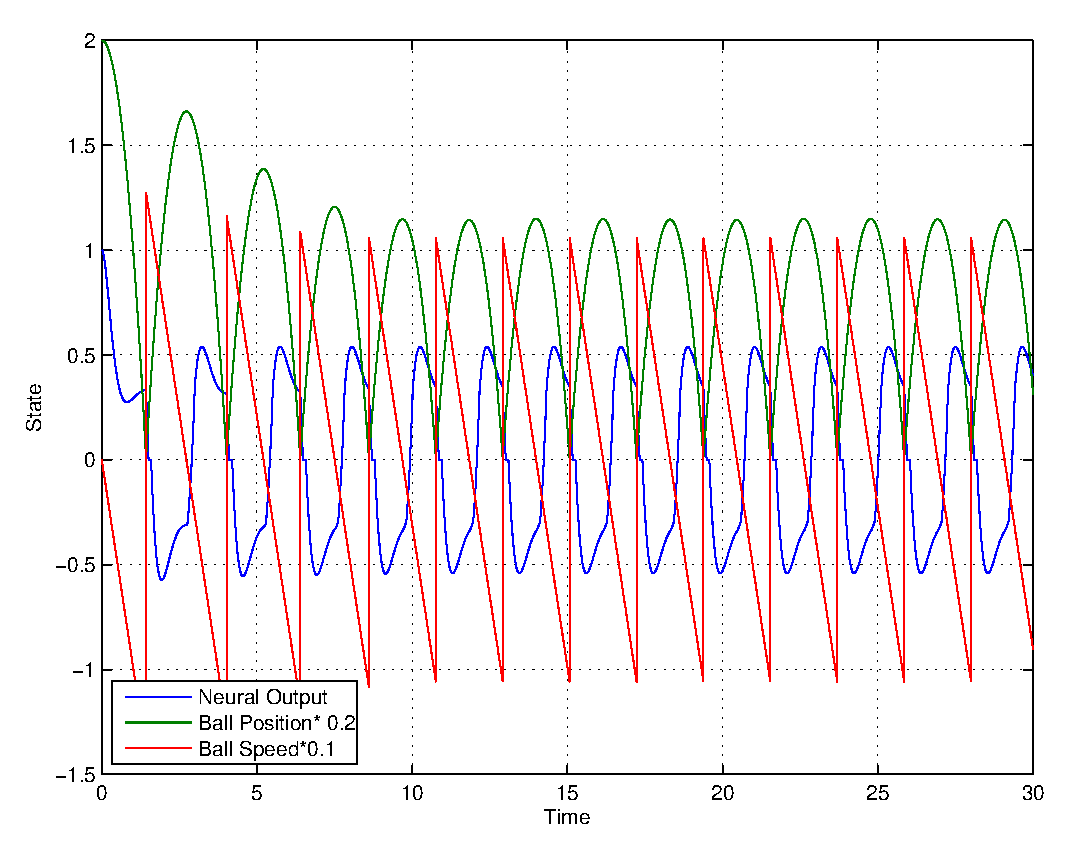
\includegraphics[width=0.45\textwidth]{\figurepath/bb_ms_os_StateTime.eps}
	\label{fig:bb_entraint}
	}
	\subfigure[Phase Plane]
	{
	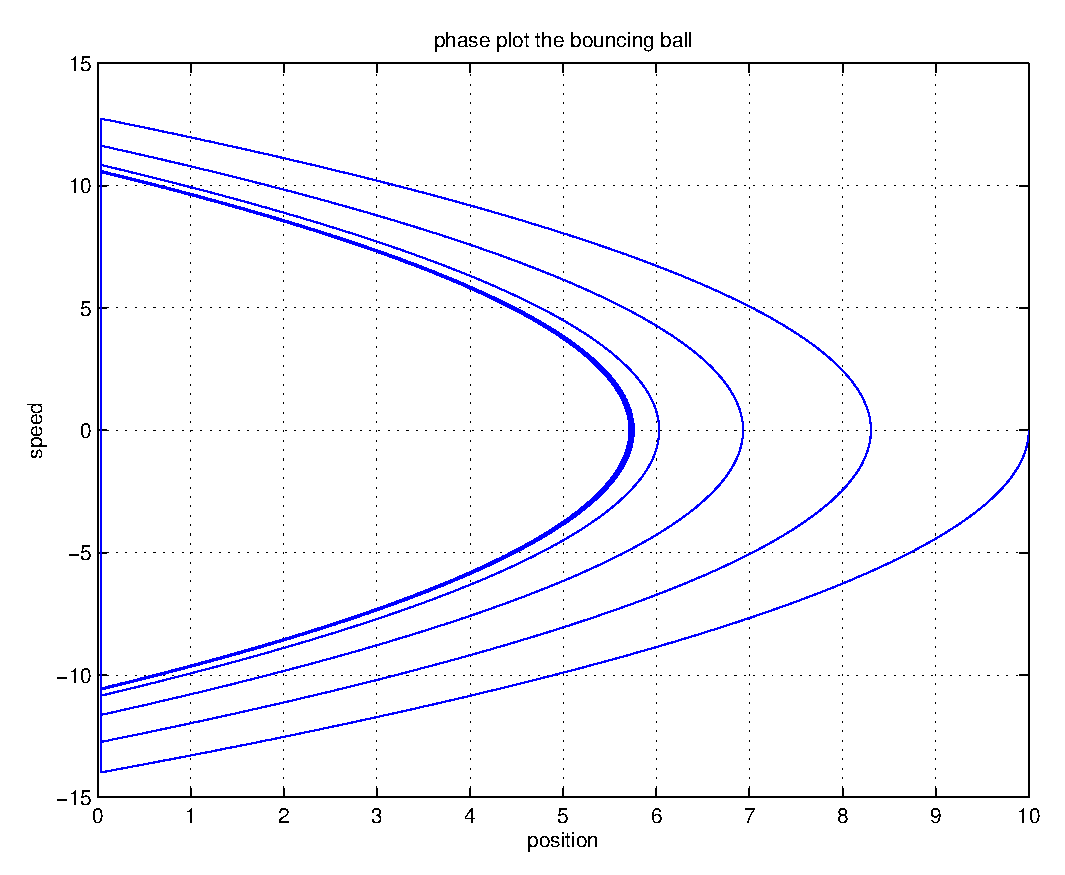
\includegraphics[width=0.45\textwidth]{\figurepath/bb_ms_os_Phase.eps}
	\label{fig:bb_entraint_phase}
	}	
\end{center}
\caption{Attractive Limited Circle}
\label{fig:fig_bb_entraint}
\end{figure}

The bouncing ball system also shows a large area of attraction. 
In Figure ~\ref{fig:bb_attractive_circle} the trajectory of the bouncing ball system converges to the same limited circle.
This means if we drop the ball from different height, after several period, 
all the balls from different drops will bouncing in the same period and reach the same height.
\begin{figure}[h]
\begin{center}
	\subfigure[state plot]
	{
	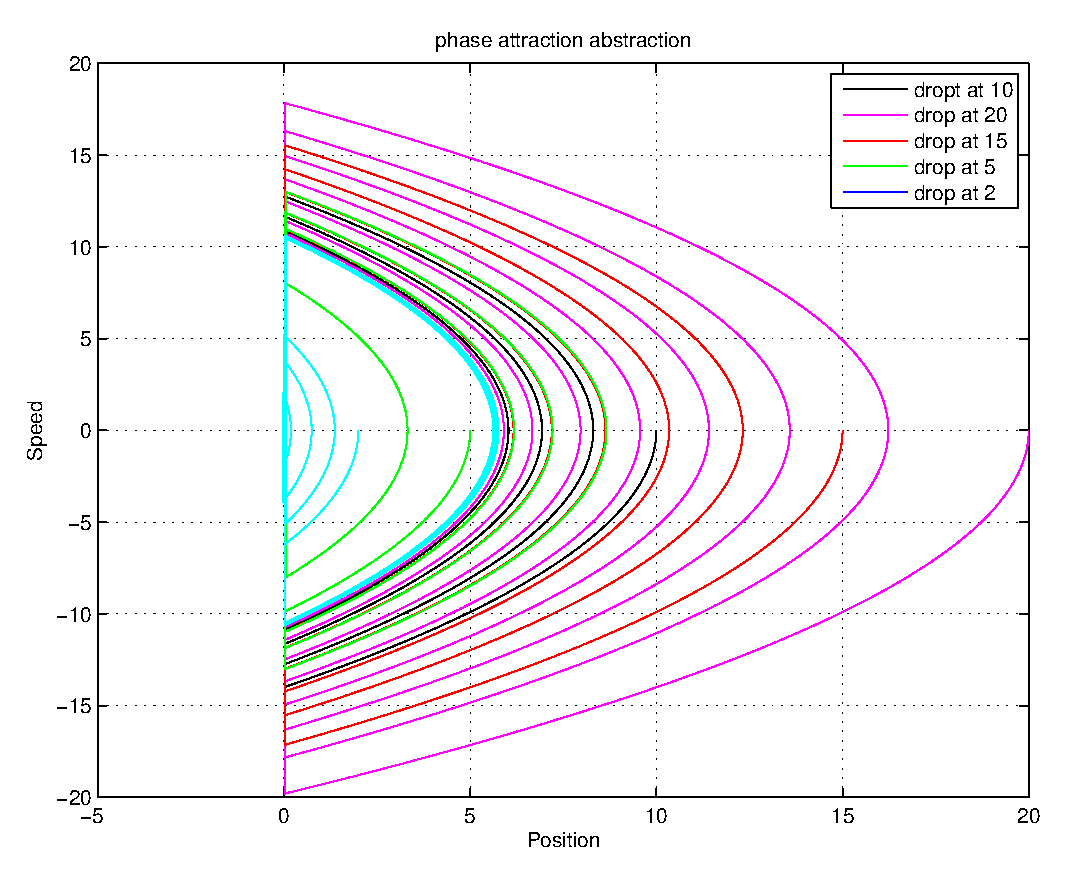
\includegraphics[width=0.45\textwidth]{\figurepath/bb_ms_os_attraction_phase.eps}
	\label{fig:bb_attractive_entraint}
	}
	\subfigure[Phase Plane]
	{
	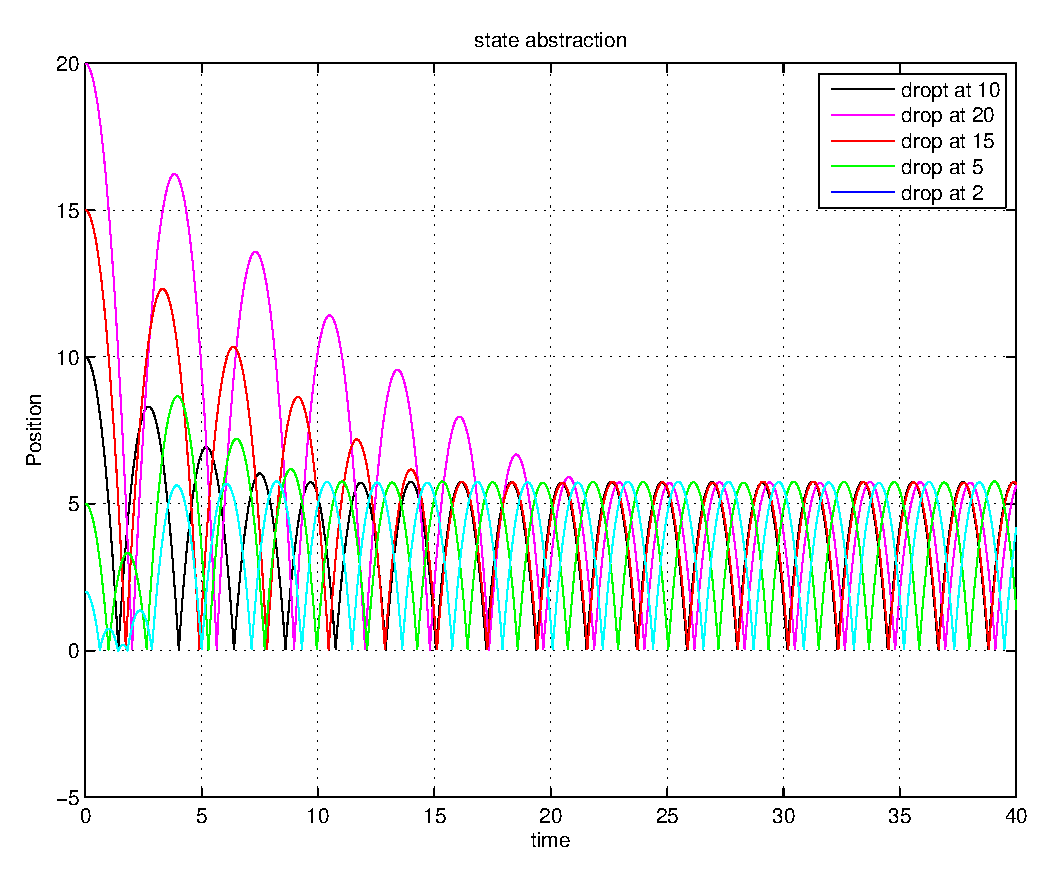
\includegraphics[width=0.45\textwidth]{\figurepath/bb_ms_os_StateTimeAttraction.eps}
	\label{fig:bb_attractive_entraint_time}
	}
	
\end{center}
\caption{Attractive Limited Circle}
\label{fig:bb_attractive_circle}
\end{figure}

\section{Passive-Based 2D walking}

Bipedal walking is a common motion task and has been well studied by many research communities, including robotic \cite{Raibert1986}, artificial intelligence and biology as well as computer graphic research.

From experience, walking involves little reasoning activity, this idea is supported by the biology research that the number of neurons that take part in the lower limb control is very limited, much less than arm, hand and even tongue.

While for artificial system, robust bipedal walking is difficult to achieve. 
Many control method has been tried, but none of them shows comparable performance with human walking. 
Among all the methods, there are two very important works:
\begin{description}
\item[ZMP]
ZMP\citep{Sugihara2002} method plans the motion curve by maintain the toppling toque zero.
Stable but slow walk has been achieved. The motion seems very rigid and looks unnatural. 
Further research shows that ZMP is not necessary or sufficient condition for walking\citep{Tedrake2008}.

\item[Passive Walking]
There have been a series of passive dynamic walking machine\citep{McGeer1990,McGeer1990a}. 
If we put a passive walking machine on a slope, without any effort, it can walk down the slop.
These systems exhibit very natural looking gaits. 
However the stabilities are very fragile. 
Passive walking can only be maintained when walking down a specific slope under specific condition.
\end{description}

From the viewport of Qualitative Control Theory, 
the reason why passive walking machines can walk down the slope is because that there exists a limit circle for the dynamic interaction between body and ground.
The fragile stability means the basin of attraction covers only a small area on the phase plane.
We plan to boost the stability of the passive walking machine by neural oscillation entrainment. 
Our method is passive-based bipedal walking.

\subsection{2D Passive Walking Machine}

The mechanical model we adopted is illustrated in Figure ~\ref{fig:2d_walker}. 
Both the model and simulation method are from the paper\citep{Wisse2005}. 
We only give brief description to make the content self-contained.

\begin{figure}
\documentclass[11pt]{article}
\usepackage{pstricks,pst-eps}
\pagestyle{empty}
\begin{document}
\begin{TeXtoEPS}
\begin{pspicture}(0,-1)(10,10)
		%\psgrid
		
		\SpecialCoor
		\psline[linestyle=dashed](!0 -10 5 sin mul)(!10 5 cos mul  -10 5 sin mul)
		%\psgrid		
		\psline[linewidth=2pt]{->}(7,8)(7,6)
		\rput(6,7){$\mathbf g$}

		%\rput(2,7)
		%{
		% $\mathbf x_{n}$,$\mathbf y_{n}$ 	
		%}
		
		\rput{-5}(0,0)
		{
			%\psgrid
			%ground
			\psline[linewidth=3pt](0,0)(10,0)
			\psarc[linewidth=0.5pt]{<-}(10,0){9}{-180}{-175}
			%\psgrid
			\rput(0.5,-0.5){$\mathbf \gamma$}
			
						
			
			%\SpecialCoor
			%\psline[linewidth=0.5pt,linestyle=dashed](!2 10 cos 8 mul)(2,0)
			%\psline[linewidth=0.5pt](2,0.5)(1.5,0.5)
			%\psline[linewidth=0.5pt](1.5,0.5)(1.5,0)
						
			\SpecialCoor
			\rput{0}(!2 10 cos 8 mul)
			{	
				\psline[linewidth=3pt,linestyle=dashed](0,0)(0,6)
				%left leg		
				\rput{10}(0,0)
				{
					%\psgrid
					
					\psline[linecolor=blue,linewidth=3pt](0,0)(0,-4)
					\pscircle(0,0){0.1}
					\rput{0}(0,-4)
					{
					\psline[linecolor=blue,linewidth=3pt](0,0)(0,-4)
					\pscircle(0,0){0.1}
					\psdots[dotstyle=Bo,dotscale=3.0](0,-2)
					}
		
				
		
					
					\psline[linewidth=0.5pt](0,0)(-2.3,0)
					\psline[linewidth=0.5pt](0,-8)(-2.3,-8)
					\psline[linewidth=0.5pt]{<->}(-2,0)(-2,-8)
					\rput(-2.2,-4){ $\mathbf L$}
		
					\psline[linewidth=0.5pt](0,-2)(-1.1,-2)	
					\psline[linewidth=0.5pt]{<->}(-1,0)(-1,-2)
					\rput(-1.2,-1.5){$\mathbf b_{2}$}

					\psline[linewidth=0.5pt](0,-4)(-1.1,-4)	
					\psline[linewidth=0.5pt]{<->}(-1,-2)(-1,-4)
					\rput(-1.2,-3.5){$\mathbf a_{2}$}


					\psdots[dotstyle=Bo,dotscale=3.0](0,-2)
					\rput(0.7,-2.2){$\mathbf m_{s}$,$\mathbf I_{s}$}


					
					\rput{-5}(0,-8)
					{
					\psline[linewidth=0.5pt,linestyle=dashed](0.1,0)(0.1,4)
					\psarc[linewidth=0.5pt,linestyle=dashed]{->}(0.1,0){3.8}{90}{95}
					\rput(0.5,4.1){$\mathbf q_{1}$}
					}
					%\psarc[linecolor=blue,linewidth=3pt](0,-6){2}{210}{330}
					
				}
				%right leg
				\rput{40}(0,0)
				{
					%\psarc[linewidth=0.5pt,linestyle=dashed]{->}(0,0){5.5}{-150}{-90}
					%\SpecialCoor	
					%\rput(6;-105){$\mathbf \phi_{2}$}	
					\psline[linecolor=red,linewidth=3pt](0,0)(0,-4)
					\pscircle(0,0){0.1}
					\psdots[dotstyle=Bo,dotscale=3.0](0,-2)
					
					\rput{-35}(0,-4)
					{
					\psline[linewidth=0.5pt,linestyle=dashed](0,0)(0,1.5)
					\psarc[linewidth=0.5pt,linestyle=dashed]{->}(0,0){1}{90}{125}
					\rput(0.3,1){$\mathbf q_{2}$}
					}
					
					\rput{-10}(0,-4)
					{
					\psline[linecolor=red,linewidth=3pt](0,0)(0,-4)
					\pscircle(0,0){0.1}

				
					\psline[linewidth=0.5pt](0,0)(1.1,0)
					\psline[linewidth=0.5pt](0,-2)(1.1,-2)	
					\psline[linewidth=0.5pt]{<->}(1,0)(1,-2)
					\rput(1.2,-1.5){$\mathbf b_{1}$}

					\psline[linewidth=0.5pt](0,-4)(1.1,-4)	
					\psline[linewidth=0.5pt]{<->}(1,-2)(1,-4)
					\rput(1.2,-3.5){$\mathbf a_{1}$}
					\psdots[dotstyle=Bo,dotscale=3.0](0,-2)
					\rput(-0.7,-2){$\mathbf m_{t}$,$\mathbf I_{t}$}
					
					\rput{-25}(0,0)
					{
						\psline[linewidth=0.5pt,linestyle=dashed](0,0)(0,-1.5)
						\psarc[linewidth=0.5pt,linestyle=dashed]{->}(0,0){1.4}{270}{295}
						\rput(-0.3,-1){$\mathbf q_{3}$}
					}
					}

				}
				\psdots[dotstyle=Bo,dotscale=3.0](0,0)
				\rput(0.7,0){$\mathbf m_{H}$}
			}
		}
\end{pspicture}
\end{TeXtoEPS}


\end{document}



\caption{Passive Walking Model}
\label{fig:2d_walker}
\end{figure}

Key parameters of the passive walker are listed below.
\[
\begin{array}{lcr}
g  &gravity   &9.81 \\
\gamma &slope angle &0.0
\end{array}
\]
The parameters of the environment is 
\[
\begin{array}{lcr}
\mbox{leg length} &l &0.4m\\
\mbox{foot radius} &r &0.1m\\
\mbox{Com Location} &c& 0.1m\\
	&w &0 m\\
\mbox{mass}& m& 1kg\\
\mbox{inertia} &I& 0.01 kgm
\end{array}
\]

In simulation, the following states are concerned.
\[
\begin{array}{ll}
X_{h} &\mbox{hip horizon displacement}\\
Y_{h}  &\mbox{hip vertical displacement}\\
\phi_{1} & \mbox{leg one angle}\\
\phi_{2} &\mbox{leg 2 angle}\\
xf_{1} &\mbox{foot location of leg1}\\
xf_{2} &\mbox{foot location of leg2}
\end{array}
\]

\subsection{ Equations of Passive Walking}
Passive walking is not a continuous dynamic system. 
We separate the motion into two phases and formulate two equations.
\begin{description}
\item[Leg Swing Phase]
During the swing phases, we suppose that one leg is fixed on the ground, the arc foot makes the passive dynamic walker rolling without sliding.
\item[Heel Strike Phase]
We suppose the heel strike the ground in a short time, the angular momentum is preserved.
\end{description}


For a two dimensional walker, every leg is determined by three variables $x_{i}$, $y_{i}$ and $\phi_{i}$. 
The number of independent variables is reduced to four, $xh$, $yh$, $\phi_{i}$, $\phi_{2}$ for the hinge joint at hip reduced two dofs. 
Then we can have the following transform or Jacobin matrix $T$.

\begin{eqnarray}
X=[x_{1},y_{1},\phi{1},x_{2},y_{2},\phi{2}]^{T} \nonumber\\
Q=[x_{h},y_{h},\phi{1},\phi{2}]^{T} \nonumber \\
X=	\left[
	\begin{array}{l}
	x_{h}+c_{1}*sin(\phi_{1})+w_{1}*cos(\phi_{1}) \\
	y_{h}-c_{1}*cos(\phi_{1})+w_{1}*sin(\phi_{1}) \\
	\phi_{1}\\
	x_{h}+c_{2}*sin(\phi_{2})+w_{2}*cos(\phi_{2})\\
	y_{h}-c_{2}*cos(\phi_{2})+w_{2}*sin(\phi_{2})\\
	\phi_{2}	
	\end{array}
	\right] 
	 \\
T_{i,k}=\frac{\delta X_{i}}{ \delta Q_{k}}  \\
T= \left[
	\begin{array}{cccc}
 	1 &0 &c_{1}*cos(\phi_{1})-w_{1}*sin(\phi_{1})&0\\
 	0 &1 &c_{1}*sin(\phi_{1})+w_{1}*cos(\phi_{1})&0\\
 	0 &0 &1 &0\\
	1 &0 &0 &c_{2}*cos(\phi_{2})-w_{2}*sin(\phi_{2})\\
	0 &1 &0 &c_{2}*sin(\phi_{2})+w_{2}*cos(\phi_{2})\\
	0 &0 &0 &1
	\end{array}\right]\\
\end{eqnarray}

By Newton and Euler's Law,

\begin{eqnarray}
F=M\ddot{x}\\
M=diag[m_{1} m_{1} I_{1} m_{2} m_{2} I_{2}]\\
F=Fg+Fc+F_{cons}
\end{eqnarray}


Combining the equations above, we have 
\[
T^{T}(F-M\ddot(x))=0
\]
\[
\ddot{x}=\dot{T \dot{q}}\\
	=T \ddot{q}+\dot{T}\dot{q}\dot{q}\\
\]
\begin{eqnarray}
g(x)&=&\dot{T} \dot{q} \dot{q}\\
	&=&
	\left[
	\begin{array}{c}
	(-c_{1}*sin(\phi_{1})-w_{1}*cos(\phi_{1}))*\dot{\phi_{1}}^2\\
	( c_{1}*cos(\phi_{1})-w_{1}*sin(\phi_{1}))*\dot{\phi_{1}}^2\\
	0\\
	(-c_{2}*sin(\phi_{2})-w_{2}*cos(\phi_{2}))*\dot{\phi_{2}}^2\\
	( c_{2}*cos(\phi_{2})-w_{2}*sin(\phi_{2}))*\dot{\phi_{2}}^2\\
	0
	\end{array}
	\right]
\end{eqnarray}


If we ignore the foot contact constraint, the equation of swinging is 
\[
\bar{M} \ddot{q}= \bar{f}
\]
\[
\bar{M}=T^{T}MT
\]
\[
\bar{f}=T^{T}[f-Mg]
\]	



Now considering the contact constraint, the position of the foot is on the ground
\[
g_{y}=y_{h}-(l-r)*cos(\phi)-r=0
\]
 and there is no slippery
\[
g_{x}=x_{h}+(l-r)*sin(\phi)+r*\phi-x_{f}
\]
\begin{equation}
D(x)=[g_{x}  g_{y}]^T=0
\end{equation}
After the first differential we get
\[
\dot{D}\dot{x}=0
\]
\[
\dot{D}=\left[
	\begin{array}{cccc} 
	1&0&(l_{1}-r_{1})*cos(\phi_{1})+r_{1}&0\\
	0&1&(l_{1}-r_{1})*sin(\phi_{1}&0
	\end{array}
	\right]
\]
After the second time differential, we have
\[
\dot{D}\dot{q}+\ddot{D}\dot{q}\dot{q}=0
\]
\[
\ddot{D}=\left[
	\begin{array}{c}
	-(l_{1}-r_{1})*sin(\phi_{1}) \dot{\phi_{1}}^2\\
	(l_{1}-r_{1})*cos(\phi_{1}) \dot{\phi_{1}}^2
	\end{array}	
\right]
\]

Putting them together, the equation for leg swing when one leg is fixed on the ground is

\begin{equation}
\left[
\begin{array}{cc}
\bar{M} &D^{T}\\
D&	0 
\end{array}
\right]
\left[
\begin{array}{c}
\ddot{q} \\
F_{c}
\end{array}
\right]
=
\left[
\begin{array}{c}
\bar{F}\\
\ddot{D}\\
\end{array}
\right]
\end{equation}

During the heel strike phase, the equation of motion is as below
\begin{equation}
\left[
\begin{array}{cc}
\bar {M}& D^{T}\\
D	& 0
\end{array}
\right]
\left[
\begin{array}{c}
\dot{q}^{+}\\
f_{c}	
\end{array}
\right]
=
\left[
\begin{array}{c}
\bar{M}\dot{q}^{-}\\
0
\end{array}
\right]
\end{equation}
where $\dot{q}_{+}$ is the state variable after the collision, $\dot{q}_{-}$ is the state variable before the collision.

\subsection{Passive Dynamic Walker Driven by Neural Oscillator}

Although the equation for 2D walking is more complex, 
in principle, 2D passive dynamic walking resembles the bouncing ball system.
Before the leg strikes the ground, it is moving passively.
Only the gravity has effects. 
This is the same with ball flying in the air. 
When the leg strikes the ground, an impulse is generated. 
The state of the system changed instantly.

The input of neural oscillator is defined by the difference angle between the two legs.
\[
G_{input}=\phi_{1}-\phi_{2}
\]
Neural output will drive the biped walker. After adding the neural control, the equation of the dynamic system is
\begin{equation}
\left[
\begin{array}{cc}
\bar{M} &D^{T}\\
D&	0 
\end{array}
\right]
\left[
\begin{array}{c}
\ddot{q} \\
F_{c}
\end{array}
\right]
=
\left[
\begin{array}{c}
\bar{F}\\
\ddot{D}
\end{array}
\right]
+
\left[
\begin{array}{c}
\bar{U}\\
0	
\end{array}
\right]
\end{equation}

Neural oscillator output is applied at the hip joint to actuate the two legs towards different directions
\[
U=[0,0,1,-1]*G_{out}
\]

\subsection{Adaptive 2D Passive-Based Walking Motion}
When the passive walker walks down a slope, for every step, there is energy input from the potential energy,
and there is also energy loss because of heel strike. 
There must be an equilibrium condition when the energy lost is equal to the energy input. 
If natural looking motion is energy efficient, such passive walking motion can be expected to be natural looking. 
Because there is no extra control energy input, such motion is the most energy efficient.

\begin{figure}[h]
\begin{center}
\includegraphics[width=0.9\textwidth]{\figurepath/passive_walking.eps}
\end{center}
\caption{Stable passive walking gait}
\label{fig:passive_walk}
\end{figure}
Figure \ref{fig:passive_walk} shows the gait of the passive walker. 
After coupling the neural oscillator, the basic pattern is not changed  as shown in Figure ~\ref{fig:stable_active_walk}.
\begin{figure}[here]
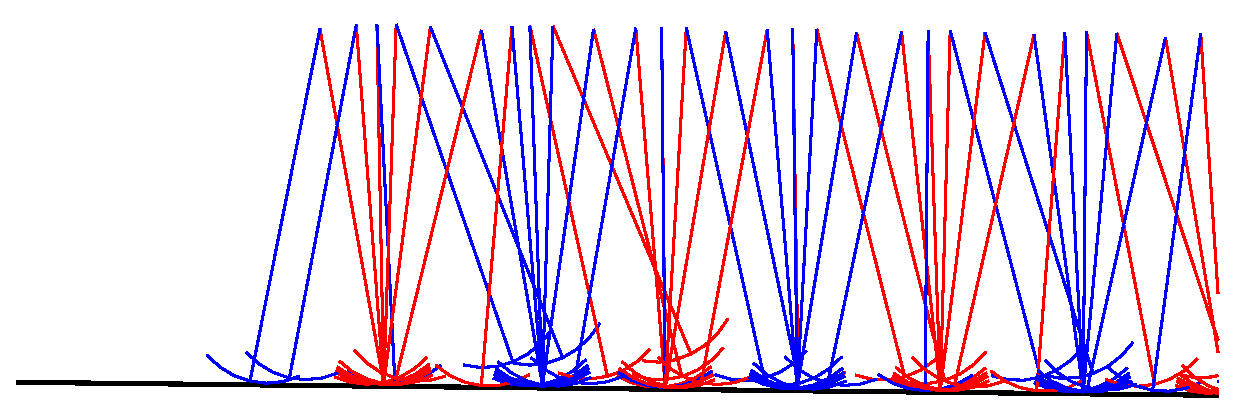
\includegraphics[width=0.9\textwidth]{\figurepath/actuated_walk_downslop.eps}
\caption{Walk down the same slop when actuated}
\label{fig:stable_active_walk}
\end{figure}

However the stability is fragile. 
On a plane ground, there is no such limited circle any more. 
The passive walker can't walk on plane. 
The step size will decrease after each step, and finally it will stop or fall over as illustrated in Figure ~\ref{fig:pass_waling_on_plane}.
\begin{figure}[here]
\begin{center}
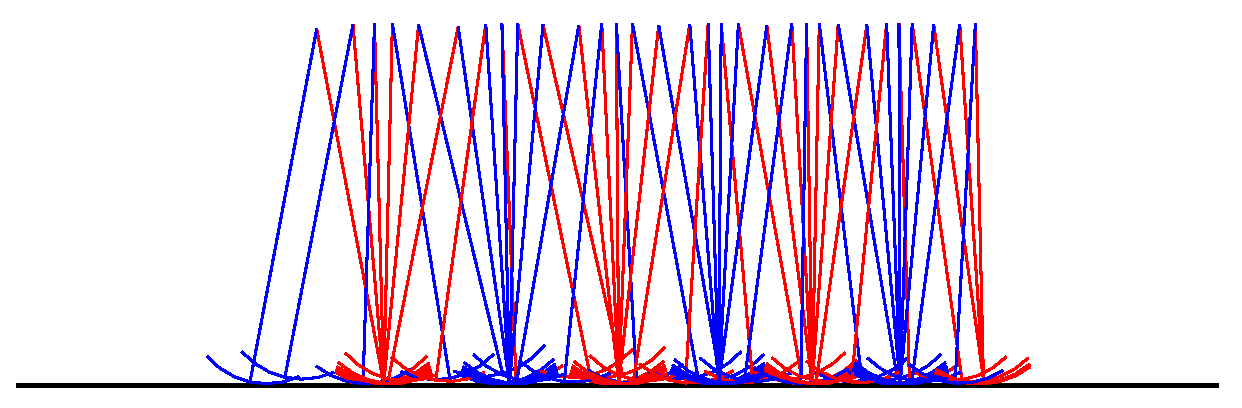
\includegraphics[width=0.9\textwidth]{\figurepath/passive_walk_on_plane.eps}
\end{center}
\caption{Passive walking gait can't be maintained on plane}
\label{fig:pass_waling_on_plane}
\end{figure}

After coupled with the neural oscillator, this walking machine can walk on plane, and exhibits gait similar to the passive dynamic walker. 
Figure ~\ref{fig:walk_plane} shows the gait. 
From the state plot Figure ~\ref{fig:walk_plane_state}, and phase plot Figure ~\ref{fig:walk_plane_phase}, we can see that the gait converged to a stable limit circle.

\begin{figure}[here]
\begin{center}
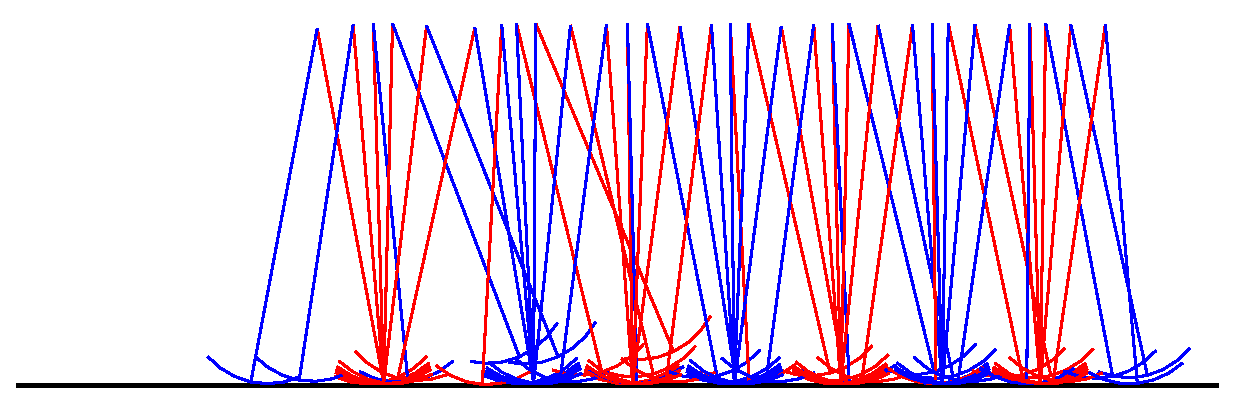
\includegraphics[width=0.9\textwidth]{\figurepath/walker_on_plane.eps}
\end{center}
\caption{Walking on plane under neural control}
\label{fig:walk_plane}
\end{figure}


\begin{figure}[here]
\begin{center}
\subfigure[State Plot]
{
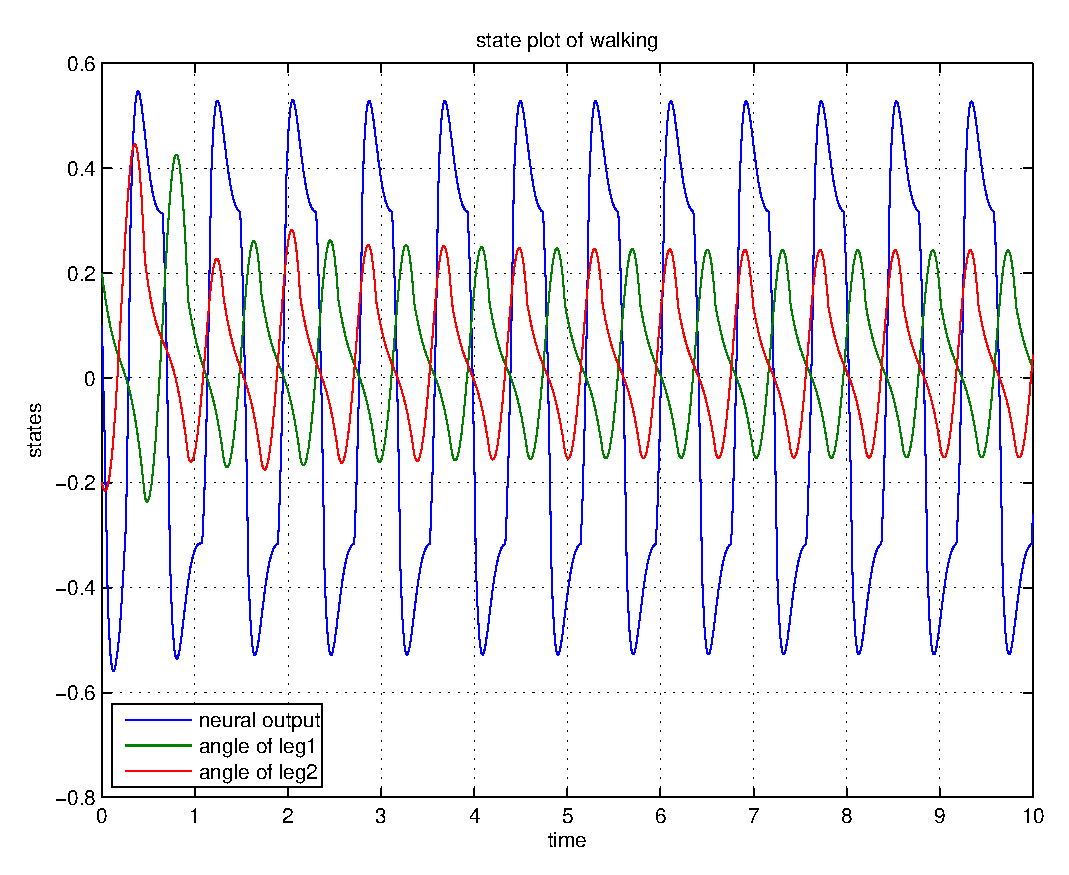
\includegraphics[height=0.45\textheight]{\figurepath/walking_on_plane_time_state}
\label{fig:walk_plane_state}
}
\subfigure[Phase Plot]
{
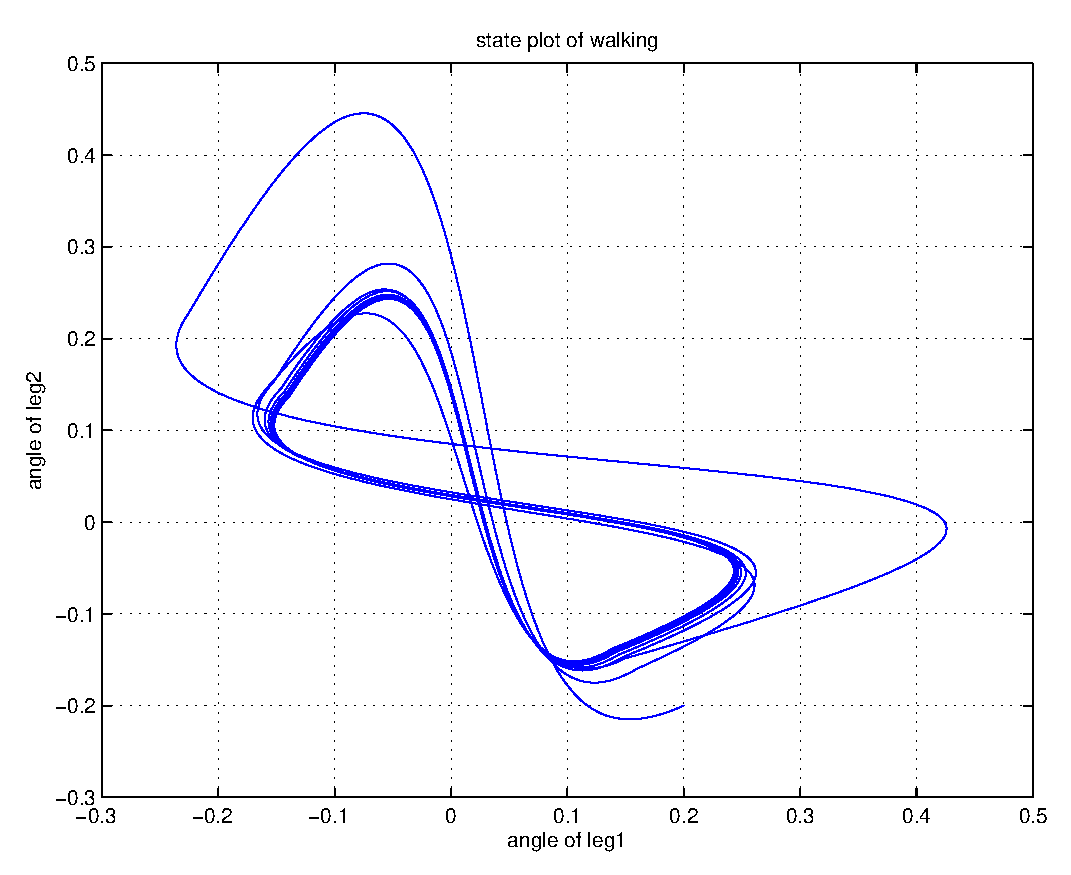
\includegraphics[height=0.45\textheight]{\figurepath/walking_on_plane_phase.eps}
\label{fig:walk_plane_phase}
}
\end{center}
\caption
{
Walking on a plane converges to a stable limited circle
}
\label{fig:walk_on_plane}
\end{figure}

To verify the structural stability, we introduce a variety of perturbations to the passive walker. 
These perturbations include different initial condition, different slopes, different leg mass and different leg length.
\begin{description}
\item [Different Initial Condition]
The original passive walker is not very stable. 
A slight change in initial condition will result in walking failure. 
While after coupled with neural oscillator, the basin of attraction has been enlarged. 
A different initial condition can still lead to a stable gait, as show in Figure \ref{fig:diff_init}. 
Natural looking gait is maintained.
\begin{figure}[here]
\begin{center}
\subfigure[without control]
{
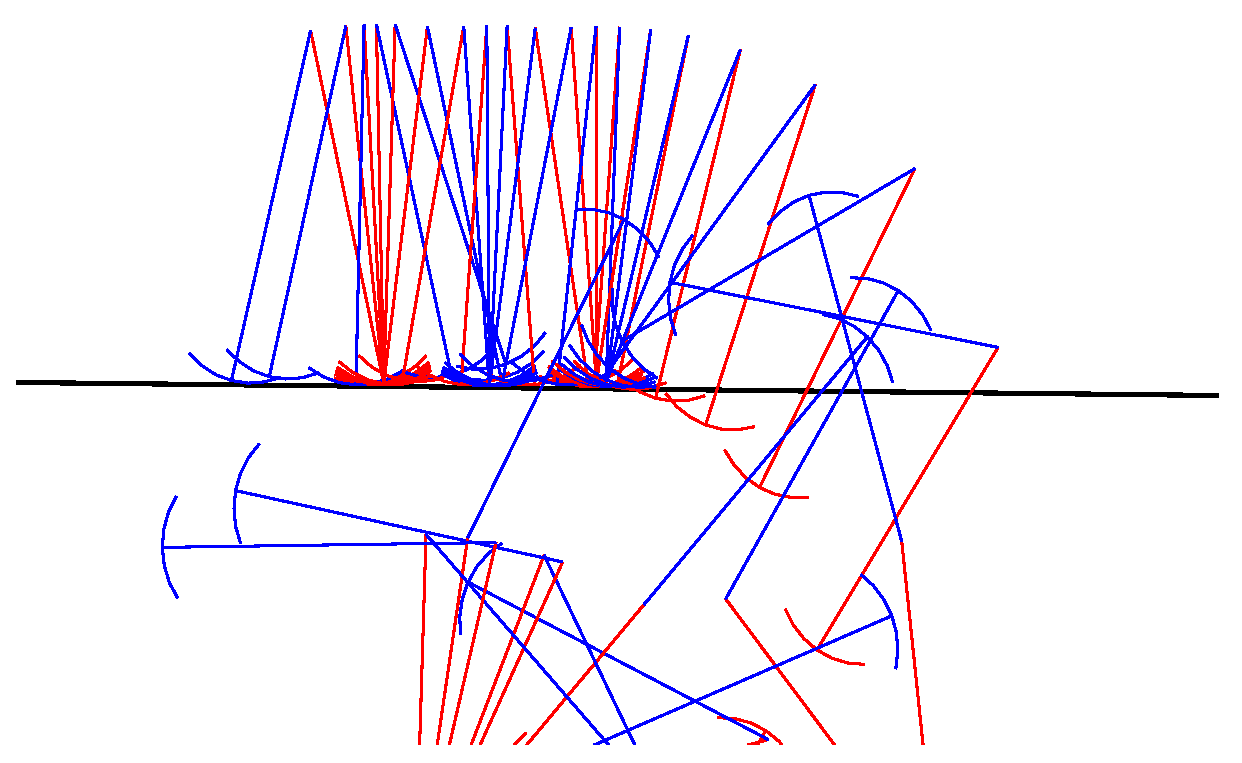
\includegraphics[width=0.9\textwidth]{\figurepath/walk_down_with_differnt_init_cond_failed.eps}
\label{fig:walk_down_different_init_failed}
}
\subfigure[with neural control]
{
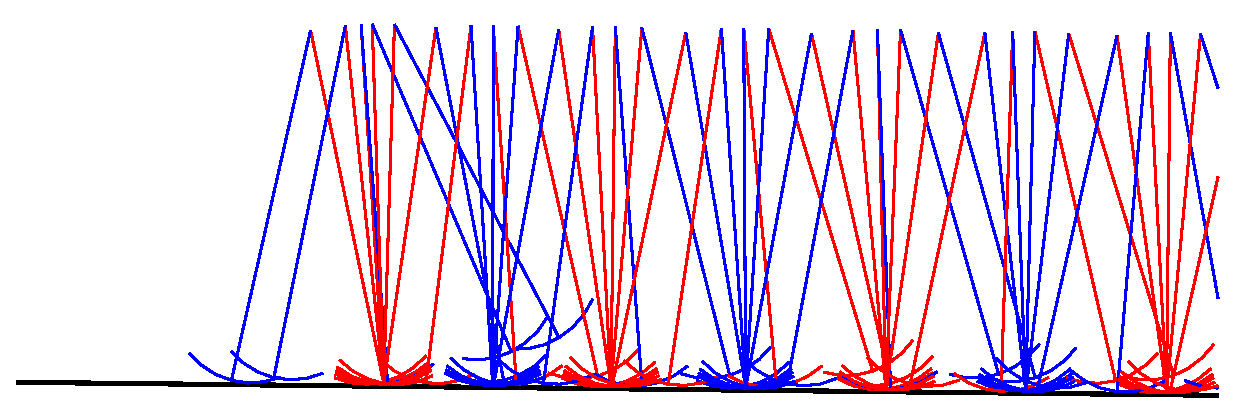
\includegraphics[width=0.9\textwidth]{\figurepath/walk_down_with_differnt_init_cond_suceed.eps}
\label{fig:walk_down_different_init_succeed}
}
\end{center}
\caption
{
Walking with different Initial condition
}
\label{fig:diff_init}
\end{figure}
 

\item[Walking On Different Slopes]
Another parameter we change is angle of the walking slope. 
When we increase the down slope, stable walking motion can still be maintained, as shown in figure \ref{fig:diff_slop}.
An important discovery is that although the walkers can walk on various down slopes, it can not walk up slope,no matter how control parameters are changed.
It can��t walk up slope and will fall backward after several steps. 
We suggest that this is because the proper limit circle does not exist in the dynamic system when walking up slope.
This finding may help us to understand the upper body effect in walking.

\begin{figure}[here]
\begin{center}
\subfigure[without control]
{
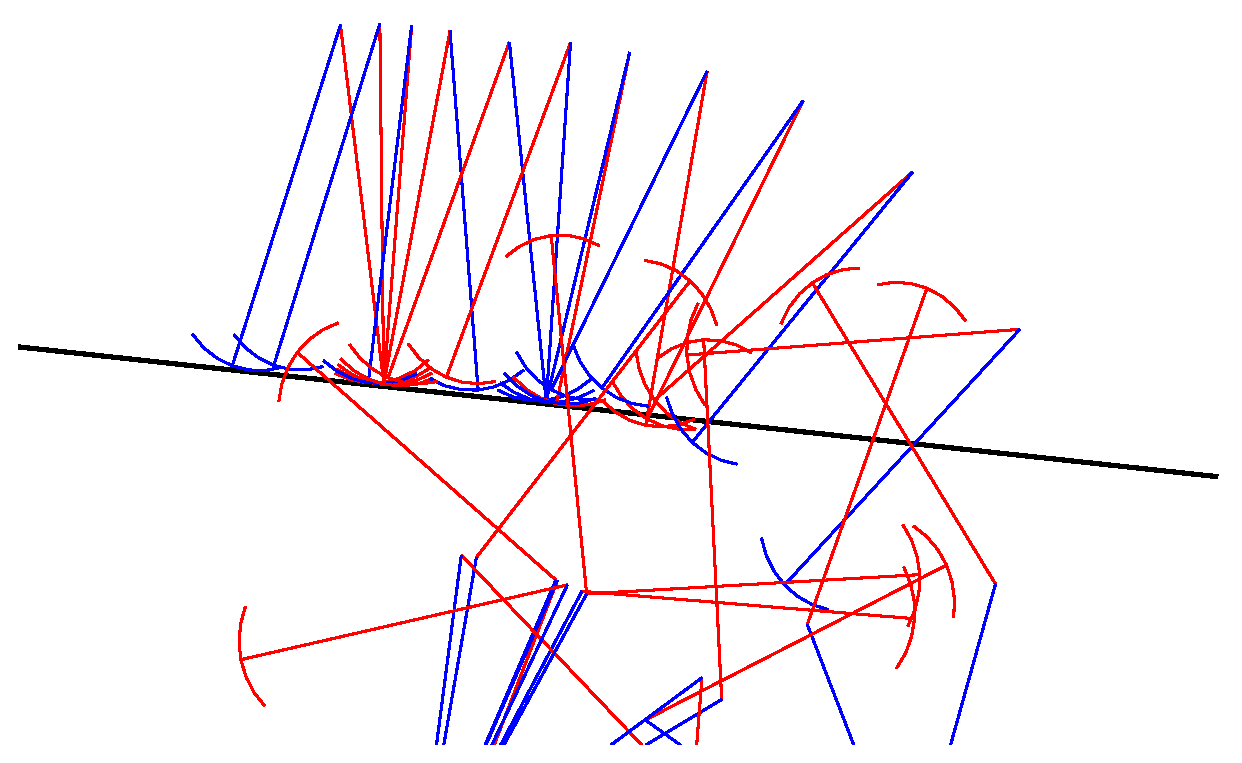
\includegraphics[width=\textwidth]{\figurepath/walk_bigger_step_failed.eps}
\label{fig:walk_bigger_slop_failed}
}
\subfigure[with neural control]
{
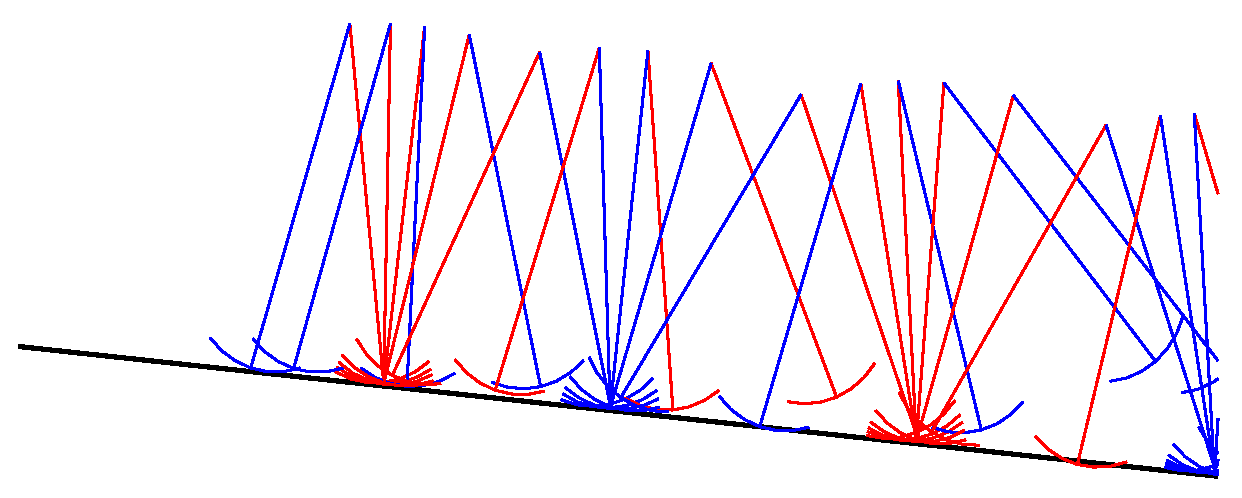
\includegraphics[width=\textwidth]{\figurepath/big_slop_actuated_suceed.eps}
\label{fig:walk_bigger_slop_succeed}
}
\end{center}

\caption
{
Walking with different slope angle
}
\label{fig:diff_slop}
\end{figure}

\item[Leg Mass Variation]
We add mass on one leg to 50\% and find the stability of the gait is still maintained. 
The step length and swing period of the two legs are different, this gait is similar to that with a crippled leg, see figure\ref{fig:leg mass}.

\begin{figure}[here]
\begin{center}
\subfigure[without control]
{
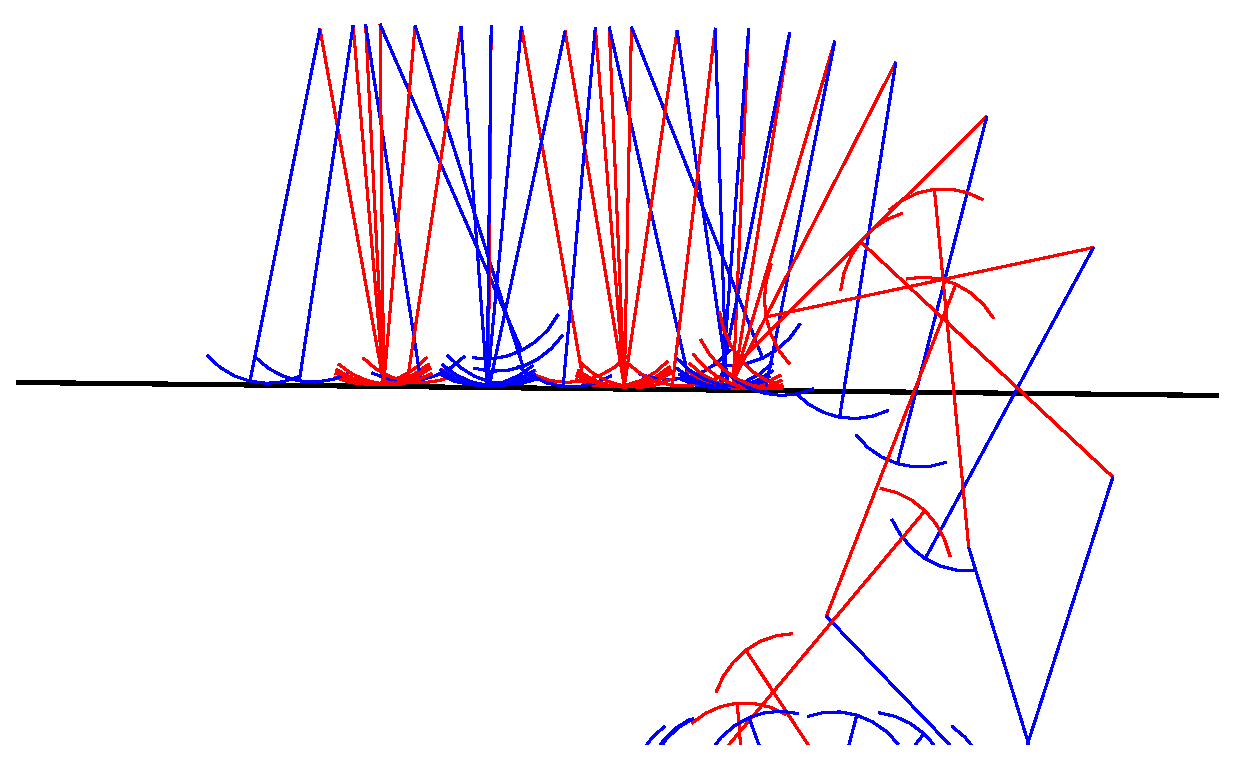
\includegraphics[width=\textwidth]{\figurepath/walk_mass_changed_passive.eps}
\label{fig:walk_mass_changed_passive}
}
\subfigure[with neural control]
{
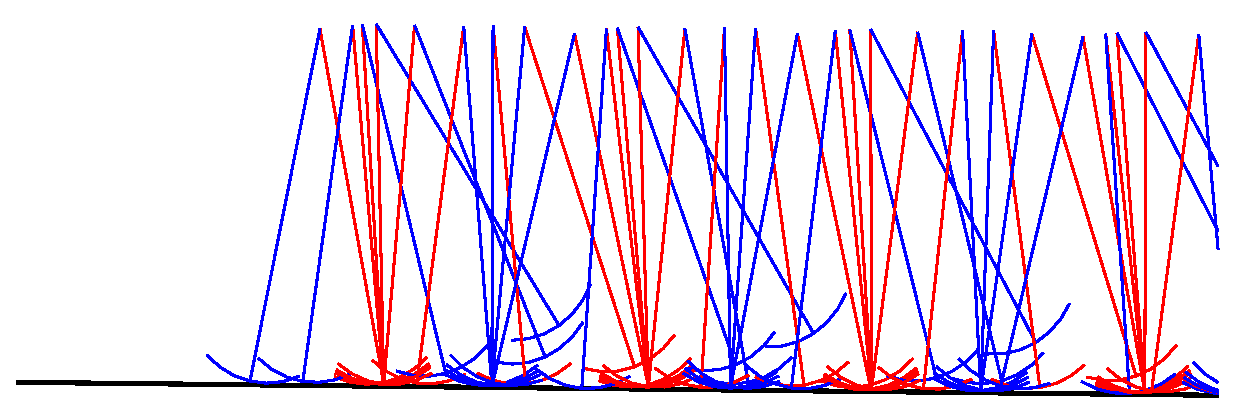
\includegraphics[width=\textwidth]{\figurepath/walk_mass_changed.eps}
\label{fig:walk_mass_changed}
}
\end{center}

\caption
{
Walking with legs of different mass
}
\label{fig:leg mass}
\end{figure}

\item[Leg Length Variation]
The last parameter we change is the leg length. 
We change the leg length to 1/8 shorter. 
And we find the stability of the gait is maintained, see Figure ~\ref{fig:walk_leg_changed}

\begin{figure}[h]
\begin{center}
\subfigure[without control]
{
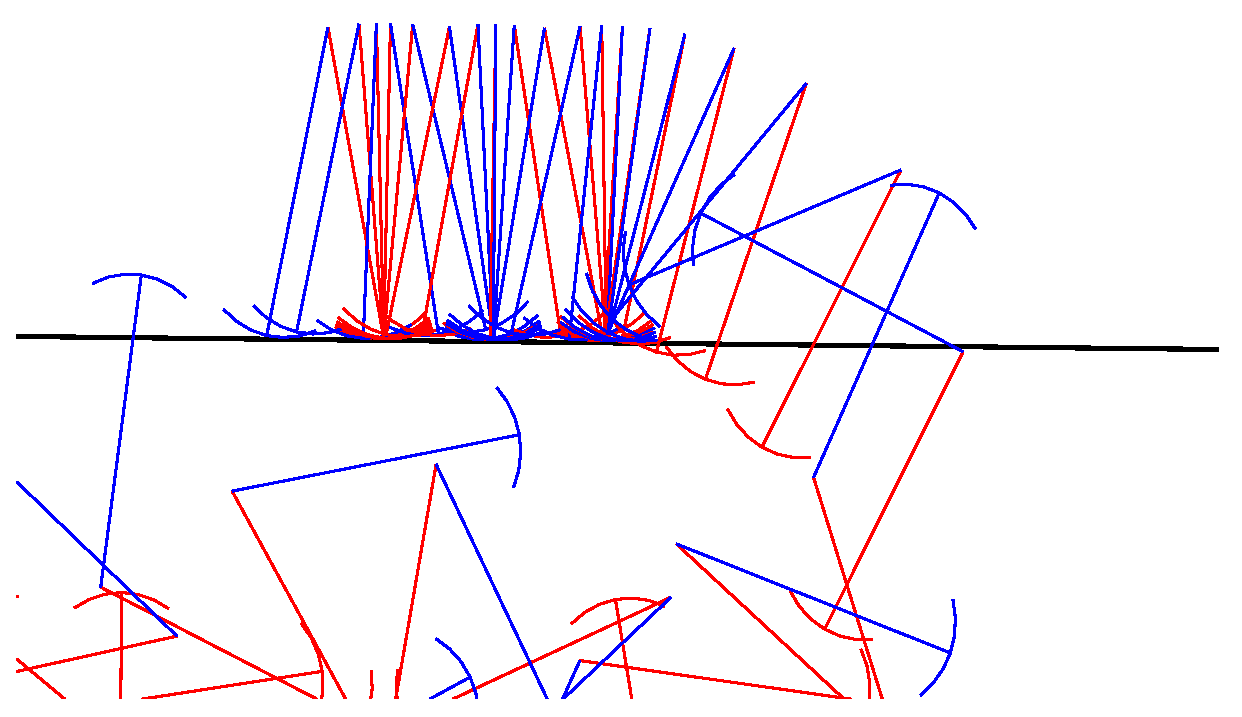
\includegraphics[width=0.8\textwidth]{\figurepath/walk_leg_changed_failed.eps}
\label{fig:walk_leg_changed_failed}
}
\subfigure[with neural control]
{
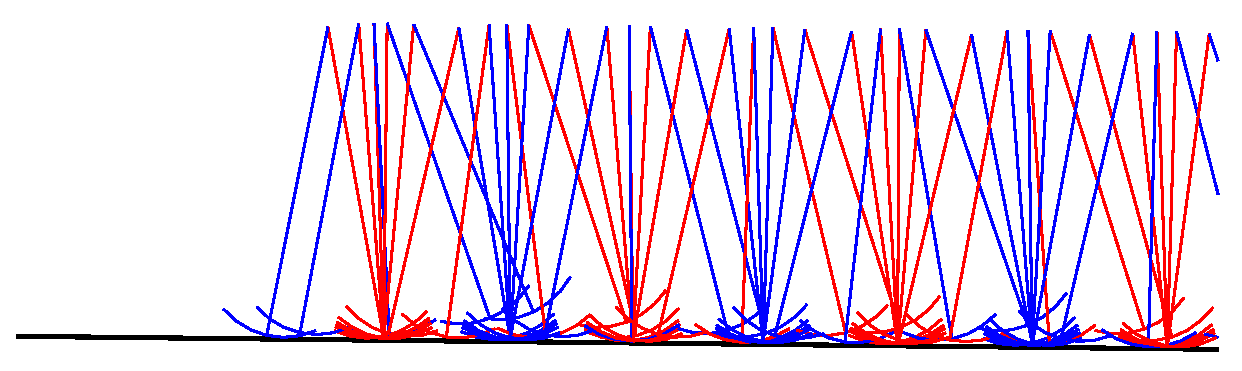
\includegraphics[width=0.8\textwidth]{\figurepath/walk_leg_changed_success.eps}
\label{fig:walk_leg_changed_sucess}
}
\end{center}

\caption
{
Walking with shorter Legs
}
\label{fig:walk_leg_changed}
\end{figure}
\end{description}

The method of nonlinear entrainment did boost the structure stability and can result in stable motion under different environment change.
By making walking a structure stable autonomous system, natural looking and adaptive motion are generated, without planning the motion curve.
%\subsection{Posture Control of An inverted Pendulum}




